% --------------------------------------------------
%  TALLER DE INTRODUCCIÓN A LaTeX
%  https://github.com/mianfg/latex-intro
%
%  Sesión 1 -> Presentación
%
%  Autor: Miguel Ángel Fernández Gutiérrez, @mianfg
%  Fecha: 20 febrero, 2019
% --------------------------------------------------

% Tipo de documento (presentación)
\documentclass[10pt, xcolor=table]{beamer}
\usepackage{caption}
\usepackage{subcaption}

% Cargar el tema
\usetheme{metropolis}

%  __________
% |          |
% | Paquetes |
% |__________|

% Paquetes de idioma
\usepackage[utf8]{inputenc}
\usepackage[spanish, es-tabla, es-lcroman, es-noquoting]{babel}

% Paquete para código fuente
% LISTINGS
\usepackage{listings}
\usepackage{lipsum}
\usepackage{courier}
\usepackage{csvsimple}

% Colores para los bloques de código
\definecolor{codegreen}{rgb}{0,0.6,0}
\definecolor{codegray}{rgb}{0.5,0.5,0.5}
\definecolor{codepurple}{rgb}{0.58,0,0.82}
\definecolor{backcolour}{rgb}{0.95,0.95,0.92}
\lstdefinestyle{mystyle}{
	backgroundcolor=\color{backcolour},   
	commentstyle=\color{codegreen},
	keywordstyle=\color{blue},
	numberstyle=\tiny\color{codegray},
	stringstyle=\color{codepurple},
	basicstyle=\footnotesize\ttfamily,
	breakatwhitespace=false,         
	breaklines=true,                 
	captionpos=b,                    
	keepspaces=true,                 
	numbers=left,                    
	numbersep=5pt,                  
	showspaces=false,                
	showstringspaces=false,
	showtabs=false,                  
	tabsize=4
}
\lstset{style=mystyle}

% Paquete de numeración en Beamer
\usepackage{appendixnumberbeamer}

% Paquete de uso para plantilla
\usepackage{booktabs}
\usepackage[scale=2]{ccicons}

% Paquete para controlar espacios
\usepackage{xspace}
\newcommand{\themename}{\textbf{\textsc{metropolis}}\xspace}

% Paquetes para matemáticas
\usepackage{amsmath}    % Paquete básico de matemáticas
\usepackage{amsthm}     % Teoremas
\usepackage{mathrsfs}   % Fuente para ciertas letras utilizadas en matemáticas

% Paquetes para fuentes
\usepackage{newpxtext, newpxmath}   % Fuente similar a Palatino
\usepackage{FiraSans}               % Fuente sans serif
\usepackage[T1]{fontenc}
\usepackage[italic]{mathastext}     % Utiliza la fuente del documento
                                    % en los entornos matemáticos

%  ________________________
% |                        |
% | Configuración del tema |
% |________________________|

% Configuración básica del tema
\metroset{
  % tema oscuro ('dark') o claro ('light'). No tiene efecto al usar la
  % paleta de colores más adelante
  background=light,
  % 'none' para eliminar la diapositiva inicial de cada sección
  sectionpage=progressbar,
  % 'progressbar' o 'simple' para añadir una diapositiva inicial a cada subsección
  subsectionpage=none,
  % contador de página: 'none', 'counter' o 'fraction'
  numbering=none,
  % barra de progreso: 'none', 'head', 'frametitle' o 'foot'
  progressbar=frametitle,
  % fondo de los bloques estilo teorema: 'transparent' o 'fill'
  block=fill,
}

% Paleta de colores
\definecolor{accent}{HTML}{009688}
\colorlet{darkaccent}{accent!70!black}
\definecolor{foreground}{RGB}{0, 0, 0}
\definecolor{background}{RGB}{255, 255, 255}

% Insertar los colores en el tema
\setbeamercolor{normal text}{fg=foreground, bg=background}
\setbeamercolor{alerted text}{fg=darkaccent, bg=background}
\setbeamercolor{example text}{fg=foreground, bg=background}
\setbeamercolor{frametitle}{fg=background, bg=accent}

\setbeamercolor{headtitle}{fg=background!70!accent,bg=accent!90!foreground}
\setbeamercolor{headnav}{fg=background,bg=accent!90!foreground}
\setbeamercolor{section in head/foot}{fg=background,bg=accent}

\defbeamertemplate*{headline}{miniframes theme no subsection}{
  % Caja para mostrar título y autor encima de cada diapositiva
  % Nosotros no 
  %% \begin{beamercolorbox}[ht=2.5ex,dp=1.125ex,
  %%     leftskip=.3cm,rightskip=.3cm plus1fil]{headtitle}
  %%   {\usebeamerfont{title in head/foot}\insertshorttitle}
  %%   \hfill
  %%   \leavevmode{\usebeamerfont{author in head/foot}\insertshortauthor}
  %% \end{beamercolorbox}
  %% \begin{beamercolorbox}[colsep=1.5pt]{upper separation line head}
  %% \end{beamercolorbox}

  % Caja para mostrar navegación encima de cada diapositiva
  \begin{beamercolorbox}{headnav}
    \vskip2pt\insertnavigation{\paperwidth}\vskip2pt
  \end{beamercolorbox}
  \begin{beamercolorbox}[colsep=1.5pt]{lower separation line head}
  \end{beamercolorbox}
}

%  _________
% |         |
% | Ajustes |
% |_________|

% Fijar tabla a posición
\usepackage{array}
\newcolumntype{L}[1]{>{\raggedright\let\newline\\\arraybackslash\hspace{0pt}}m{#1}}
\newcolumntype{C}[1]{>{\centering\let\newline\\\arraybackslash\hspace{0pt}}m{#1}}
\newcolumntype{R}[1]{>{\raggedleft\let\newline\\\arraybackslash\hspace{0pt}}m{#1}}

%  ________
% |        |
% | Título |
% |________|

\title{Algoritmos Greedy (o voraces)}
\subtitle{Algorítmica. \alert{Práctica 3}}
\date{Mayo 2022}
\author{Jose Alberto Hoces Castro\\Javier Gómez López\\ Manuel Moya Martín Castaño\\[4pt]}
\titlegraphic{\hfill
\includegraphics[width=2.5cm]{logo_dark.jpg}}

%  ___________
% |           |
% | Documento |
% |___________|

\begin{document}
\maketitle

\begin{frame}{Contenidos}
	\setbeamertemplate{section in toc}[sections numbered]
	\tableofcontents[]
\end{frame}

\begin{frame}[fragile]{Objetivo de la práctica}
	Aprender a analizar un problema y resolverlo mediante la técnica Greedy, además de justificar su utilidad para resolver problemas de forma muy eficiente, obteniendo la solución óptima o muy cercana a la óptima.
\end{frame}

\section{Ejercicio 1. Contenedores}
\begin{frame}[fragile]{Enunciado}
	\textit{Se tiene un buque mercante cuya capacidad de carga es de } K \textit{toneladas y un conjunto de contenedores \(c_1, \dotsc, c_n\) cuyos pesos respectivos son \(p_1, \dotsc, p_n\) (expresados también en toneladas). Teniendo en cuenta que la capacidad del buque es menor que la suma total de los pesos de los contenedores: }
\end{frame}

\begin{frame}[fragile]{Primer ejercicio}
	\textit{Diseñe un algoritmo que maximice el número de contenedores cargados, y demuestre su optimalidad.}
\end{frame}

\begin{frame}[fragile]{Primer ejercicio. \normalfont{Planteamiento del algoritmo}}
	\begin{itemize}
		\item Como queremos cargar el máximo número de contenedores, empezaremos cargando los más \textbf{pequeños}.
		\item Ordenamos de \textbf{menor a mayor} peso los contenedores.
		\item Empezamos a cargar los de menor peso hasta que superemos las K toneladas del buque mercante.
		\item Todo esto lo simulamos con un vector de enteros en nuestro código, el cual tenemos a continuación.
	\end{itemize}
\end{frame}

\begin{frame}[fragile]{Primer ejercicio. \normalfont{Código}}
	\lstinputlisting[language=C++]{./Codes/contenedores1.cpp}
\end{frame}

\begin{frame}[fragile]{Primer ejercicio. \normalfont{Enfoque Greedy}}
	Las 6 características de nuestro problema que hacen que lo identifiquemos como problema Greedy son:
	\begin{itemize}
		\item \textbf{Un conjunto de candidatos}: En este caso, los contenedores a cargar.
		\item \textbf{Una lista de candidatos ya usados}: Los contenedores que ya han sido cargados.
		\item \textbf{Un criterio que dice cuándo un conjunto de candidatos forma una solución}: El criterio es que la suma de los pesos de un conjunto de contenedores no sea superior a las K toneladas del buque.
	\end{itemize}
	
\end{frame}

\begin{frame}[fragile]{Primer ejercicio. \normalfont{Enfoque Greedy}}
	\begin{itemize}
		\item \textbf{Un criterio que dice cuándo un conjunto de candidatos es factible (podrá llegar a ser una solución)}: el conjunto de contenedores que se evalúe no debe superar en peso las K toneladas del buque.
		\item \textbf{Una función de selección que indica en cualquier instante cuál es el candidato más prometedor de los no usados todavía}: El contenedor de menor peso de los que aún no están cargados, de ahí que los ordenemos de menor a mayor peso.
		\item \textbf{La función objetivo que intentamos optimizar}: El número de contenedores a cargar, es lo que queremos maximizar.
	\end{itemize}
	
\end{frame}


\begin{frame}[fragile]{Primer ejercicio. \normalfont{Estudio de la optimalidad}}
	
	Sea $T = \lbrace c_{1},...,c_{n} \rbrace$ y llamemos $S = \lbrace c_{1},...,c_{m} \rbrace$ a la solución de nuestro algoritmo Greedy.
	
	\[
	\sum_{c_{i} \in S}p_{i} = \sum_{i = 1}^{m}p_{i} \leq  K \hspace{0.2cm} \text{y} \hspace{0.2cm} \sum_{i = 1}^{m+1}p_{i} > K
	\]
	
	Sea $U \subset T$ con un número mayor de contenedores que $S$ y veamos que no es solución, es decir, que $\sum_{c_{i} \in U}p_{i} > K$.
\end{frame}

\begin{frame}[fragile]{Primer ejercicio. \normalfont{Estudio de la optimalidad}}
	
	\[
	\sum_{c_{i} \in U}p_{i} = \sum_{c_{i} \in S \cap U}p_{i} + \sum_{c_{i} \in U \setminus S}p_{i}
	\]
	\centering $\downarrow$
	\[
	\sum_{c_{i} \in S \cap U}p_{i} + \sum_{c_{i} \in U \setminus S}p_{i} = \sum_{c_{i} \in S \cap U}p_{i} + \sum_{c_{i} \in R}p_{i} + \sum_{c_{i} \in U \setminus S \setminus R}p_{i}
	\]
	\centering $\downarrow$
	\[
	\sum_{c_{i} \in S \cap U}p_{i} + \sum_{c_{i} \in R}p_{i} + \sum_{c_{i} \in U \setminus S \setminus R}p_{i} \geq \sum_{c_{i} \in S \cap U}p_{i} + \sum_{c_{i} \in S \setminus U}p_{i} + \sum_{c_{i} \in U \setminus S \setminus R}p_{i}
	\]
	\centering $\downarrow$
	\[
	\sum_{c_{i} \in S \cap U}p_{i} + \sum_{c_{i} \in S \setminus U}p_{i} + \sum_{c_{i} \in U \setminus S \setminus R}p_{i} = \sum_{c_{i} \in S}p_{i} + \sum_{c_{i} \in U \setminus S \setminus R}p_{i} > K
	\]
	
	Luego hemos demostrado que $\sum_{c_{i} \in U}p_{i} > K$ y por lo tanto, $U$ no es solución.
	
\end{frame}
	
\begin{frame}[fragile]{Segundo ejercicio}
	\textit{Diseñe un algoritmo que intente maximizar el número de toneladas cargadas.}
\end{frame}

\begin{frame}[fragile]{Segundo ejercicio. \normalfont{Planteamiento del algoritmo}}
	\begin{itemize}
		\item Como queremos cargar el máximo número de toneladas, empezaremos cargando los más \textbf{pesados}.
		\item Ordenamos de \textbf{mayor a menor} peso los contenedores.
		\item Empezamos a cargar los de mayor peso hasta que superemos las K toneladas del buque mercante.
		\item Todo esto lo simulamos con un vector de enteros en nuestro código, el cual tenemos a continuación.
	\end{itemize}
\end{frame}

\begin{frame}[fragile]{Segundo ejercicio. \normalfont{Código}}
	\lstinputlisting[language=C++]{./Codes/contenedores2.cpp}
\end{frame}

\begin{frame}[fragile]{Segundo ejercicio. \normalfont{Estudio de la optimalidad}}
	\centering [5, 4, 6, 1, 1, 2, 7, 9, 8, 3] \hspace{0.2cm}K = 10
	\\
	\centering $\downarrow$
	\\
	\centering [9, 8, 7, 6, 5, 4, 3, 2, 1, 1]
	\\
	\textbf{Solución aportada por nuestro algoritmo}: [9]
	\\
	\textbf{Solución óptima}: [1,2,3,4]
	
\end{frame}

\section{Ejercicio 2. El problema del viajante de comercio}

\begin{frame}[fragile]{Enunciado}
\textit{Dado un conjunto de ciudades y una matriz con las distancias entre todas ellas, un viajante debe recorrer todas las ciudades exactamente una vez, regresando al punto de partida de forma tal que la distancia recorrida sea mínima.}
\end{frame}

\begin{frame}[fragile]{TSP. \normalfont{Heurística del vecino más cercano}}
\begin{enumerate}
	\item Partimos de un nodo cualquiera.
	\item Encontramos el nodo más cercano a este nodo, y lo añadimos al recorrido.
	\item Repetimos el proceso hasta cubrir todos los nodos.
\end{enumerate}
\end{frame}

\begin{frame}[fragile]{Heurística del vecino más cercano. \normalfont{Código}}
\begin{center}
\scalebox{0.75}{
\lstinputlisting[language=Python]{./Codes/cercania.py}
}
\end{center}
\end{frame}

\begin{frame}[fragile]{Heurística del vecino más cercano. \normalfont{Análisis Teórico}}
\[
	T(n) \in \mathcal{O} (n^2)
\]
\end{frame}

\begin{frame}[fragile]{Heurística del vecino más cercano. \normalfont{Análisis empírico}}
\begin{table}[h!]
 	\centering
 	\footnotesize
 	\scalebox{0.6}{
 		\begin{tabular}{|c|c|}
 			\hline
 			\multicolumn{2}{|c|}{\textsf{Heurística del Vecino más cercano}}
 			\\\hline
 			\bfseries Ciudades (n) & \bfseries Tiempo (s)
 			\csvreader{./data/cercania.csv}{}
 			{\\\hline\csvcoli&\csvcolii}
 			\\\hline
 		\end{tabular}
 	}
 	\caption{Experiencia empírica de el vecino más cercano}
 \end{table}
\end{frame}

\begin{frame}[fragile]{Heurística del vecino más cercano. \normalfont{Análisis Híbrido}}
 \begin{figure}[h!]
 	\centering
 	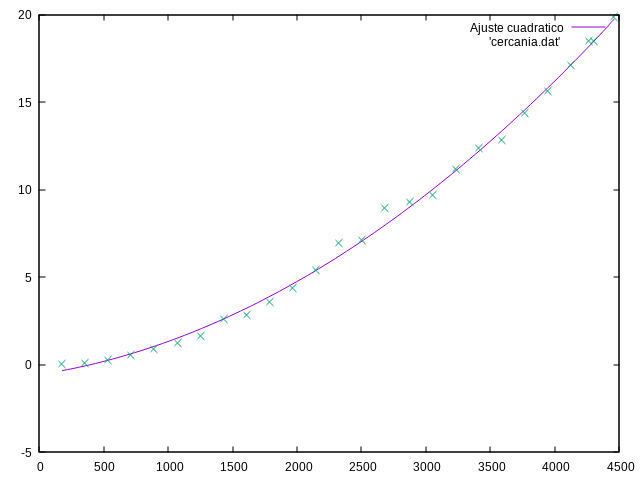
\includegraphics[scale=0.5]{./Images/cercania.png}
 	\caption{Gráfica con los tiempos de ejecución del vecino más cercano. \(R^2 = 0.869828\)}
 \end{figure}
\end{frame}

\begin{frame}[fragile]{Heurística del vecino más cercano. \normalfont{Resultados}}
\begin{itemize}
	\item \texttt{ulysses16.tsp}:
	\[
		[0,7,15,12,11,13,6,5,14,4,8,9,3,1,2,10] \qquad D = 103
	\]

	\item \texttt{bayg29.tsp}:
	\[
		[0,27,5,11,8,4,20,1,19,9,3,14,17,13,21,16,10,18,24,
	\]
	\[
		6,22,26,7,23,15,12,28,25,2] \qquad D = 10209
	\]
	
	\item \texttt{eil76.tsp}:
	\[
		[0,72,32,62,15,2,43,31,8,38,71,57,9,37,64,10,65,52,13,18,34,6,7,45,
	\]
	\[
		33,51,26,44,28, 47,46,20,73, 27, 61,1,29,3,74,75,
	\]
	\[
		66,25,11,39,15,50,5,67,4,36,19,69,59,70,35,68,60,2,1,
	\]
	\[
		41,40,42,22,55,48,23,17,49,24,54,30,58,53,12,56,14,63] \qquad D = 642
	\]
\end{itemize}
\end{frame}

\begin{frame}[fragile]{Heurística del vecino más cercano. \normalfont{Gráficos}}
\begin{center}
\begin{tabular}{cc}
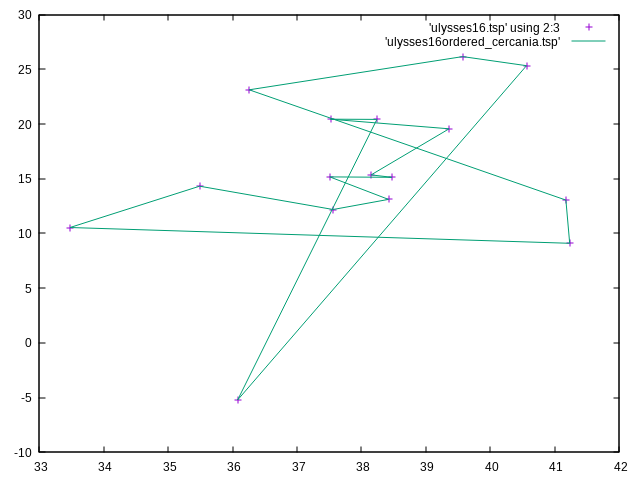
\includegraphics[scale=0.23]{./Images/ulysses_cercania.png}
&
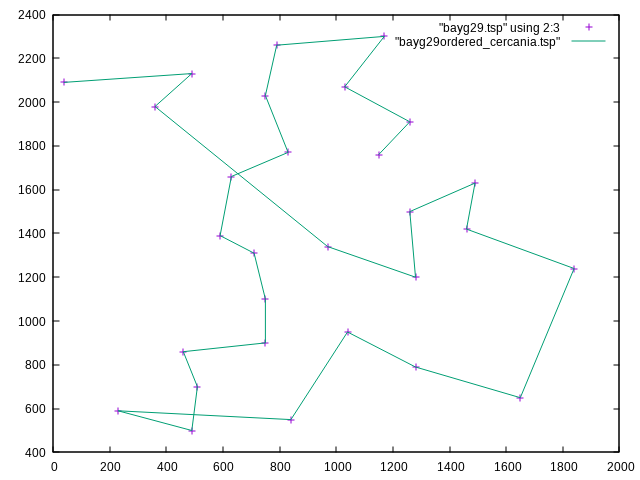
\includegraphics[scale=0.23]{./Images/bayg_cercania.png} \\
Ulysses & Bayg
\end{tabular}
\end{center}
\begin{center}
\begin{tabular}{c}
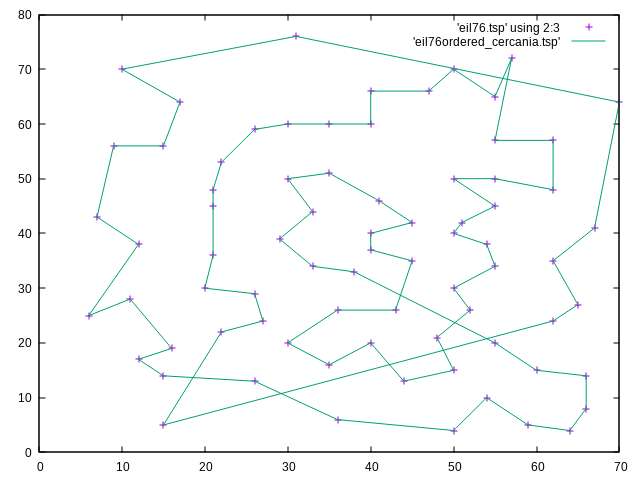
\includegraphics[scale=0.23]{./Images/eil_cercania.png} \\
Eil
\end{tabular}
\end{center}
\end{frame}

\begin{frame}[fragile]{TSP. \normalfont{Heurística de inserción}}
Veamos las 6 características de nuestro problema Greedy:
	\begin{itemize}
		\item \textbf{Un conjunto de candidatos}: En este caso, las ciudades por las que pasar.
		\item \textbf{Una lista de candidatos ya usados}: Los ciudades por las que ya se ha pasado. Cabe resaltar que se debe comenzar por un recorrido inicial de 3 ciudades previamente. Para escoger estas ciudades simplemente lo haremos escogiendo la ciudad más al oeste, la más al este y la más al norte.
		\item \textbf{Un criterio que dice cuándo un conjunto de candidatos forma una solución}: El criterio es que el recorrido que se haga forme un circuito pasando por todas las ciudades una sola vez.
		\item \textbf{Un criterio que dice cuándo un conjunto de candidatos es factible (podrá llegar a ser una solución)}: En caso de que no se repita ningún nodo (ciudad), el conjunto de candidatos es factible.
		\end{itemize}
		
\end{frame}
\begin{frame}[fragile]{TSP. \normalfont{Heurística de inserción}}
	\begin{itemize}
	
		\item \textbf{Una función de selección que indica en cualquier instante cuál es el candidato más prometedor de los no usados todavía}: Utilizaremos un criterio que denominaremos inserción mas económica: de entre todas las ciudades no visitadas, elegimos aquella que provoque el menor incremento en la longitud total del circuito.
En otras palabras, cada ciudad debemos insertarla en cada una de las soluciones posibles y quedarnos con la ciudad (y posición) que nos permita obtener un circuito de menor longitud. Seleccionaremos aquella ciudad que nos proporcione el mínimo de los mínimos calculados para cada una de las ciudades
		\item \textbf{La función objetivo que intentamos optimizar}: El coste del recorrido total del circuito.
\end{itemize}
\end{frame}

\begin{frame}[fragile]{Heurística de inserción. \normalfont{Código}}
\begin{center}
\scalebox{0.75}{
\lstinputlisting[language=C++]{./Codes/pseudocodigo_insercion.cpp}
}
\end{center}
\end{frame}

\begin{frame}[fragile]{Heurística de inserción. \normalfont{Análisis Teórico}}
\[
	T(n) \in \mathcal{O} (n^3)
\]
\end{frame}

\begin{frame}[fragile]{Heurística de inserción. \normalfont{Análisis empírico}}
\begin{table}[h!]
 	\centering
 	\footnotesize
 	\scalebox{0.6}{
 		\begin{tabular}{|c|c|}
 			\hline
 			\multicolumn{2}{|c|}{\textsf{Heurística de inserción}}
 			\\\hline
 			\bfseries Ciudades (n) & \bfseries Tiempo (s)
 			\csvreader{./data/insercion.csv}{}
 			{\\\hline\csvcoli&\csvcolii}
 			\\\hline
 		\end{tabular}
 	}
 	\caption{Experiencia empírica de inserción}
 \end{table}
\end{frame}

\begin{frame}[fragile]{Heurística de inserción. \normalfont{Análisis Híbrido}}
 \begin{figure}[h!]
 	\centering
 	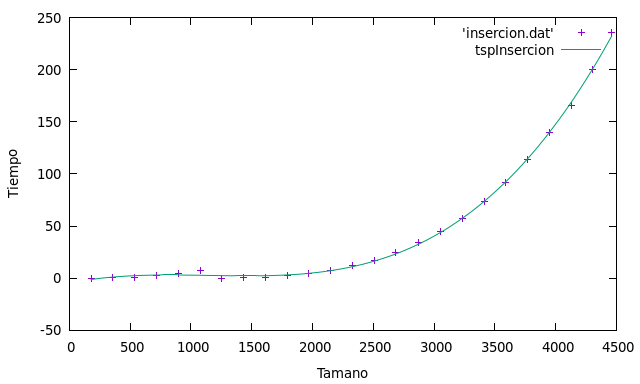
\includegraphics[scale=0.5]{./Images/insercion.png}
 	\caption{Gráfica con los tiempos de ejecución de insercion. \(R^2 = 0.85647\)}
 \end{figure}
\end{frame}

\begin{frame}[fragile]{Heurística de inserción. \normalfont{Resultados}}
\begin{itemize}
	\item \texttt{ulysses16.tsp}:
	\[
		[5, 6, 7, 10, 12, 14, 15, 13, 16, 1, 4, 8, 9, 11, 2, 3]	\qquad D = 99
	\]		

	\item \texttt{bayg29.tsp}:
	\[
		[3, 23, 12, 6, 5, 26, 29, 21, 2, 20, 10, 13, 4, 15, 19, 25, 7, 18,
		\]
		\[
		 14, 22, 11, 17, 9, 28, 1, 24, 27, 16, 8] \qquad D = 10048
	\]
	
	\item \texttt{eil76.tsp}:
	\[
		[56, 23, 63, 33, 73, 62, 22, 28, 61, 74, 30, 48, 5, 15, 57, 37, 20, 70, 60,
	\]
	\[
	 71, 47, 36, 69, 21, 29, 45, 27, 13, 54, 52, 34, 67, 26, 76, 75, 4, 68, 6, 51,
	 \]
	\[
	 17, 12, 40, 46, 8, 35, 53, 11, 66, 65, 38, 10, 58, 72, 39, 9, 32, 50, 25, 55,
	 \]
	\[
	 18, 44, 3, 14, 19, 7, 2, 1, 43, 41, 42, 64, 16, 49, 24, 59, 31] \qquad D = 611
	\]
\end{itemize}
\end{frame}

\begin{frame}[fragile]{Heurística de insercion. \normalfont{Gráficos}}
\begin{center}
\begin{tabular}{cc}
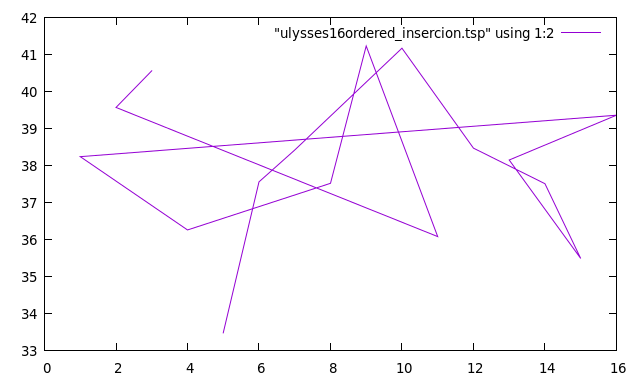
\includegraphics[scale=0.23]{./Images/ulysses_insercion.png}
&
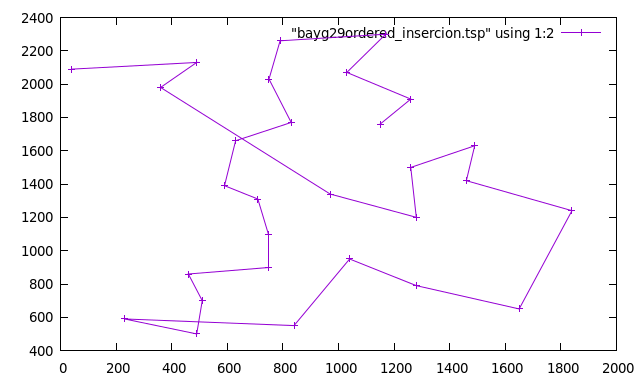
\includegraphics[scale=0.23]{./Images/bayg_insercion.png} \\
Ulysses & Bayg
\end{tabular}
\end{center}
\begin{center}
\begin{tabular}{c}
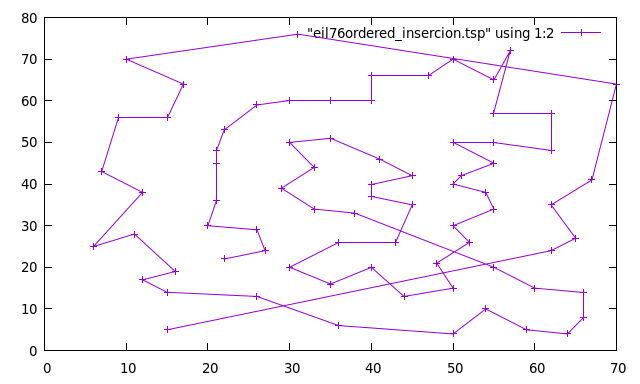
\includegraphics[scale=0.23]{./Images/eil_insercion.png} \\
Eil
\end{tabular}
\end{center}
\end{frame}

\begin{frame}[fragile]{TSP. \normalfont{Heurística de perturbaciones}}
Este enfoque, de nuevo \textit{greedy}, realiza las perturbaciones indicadas por un parámetro sobre un recorrido dado para intentar mejorarlo. 
\end{frame}

\begin{frame}[fragile]{Heurística de perturbaciones. \normalfont{Código}}
\begin{center}
\scalebox{0.7}{
\lstinputlisting[language=Python]{./Codes/perturbaciones.py}
}
\end{center}
\end{frame}

\begin{frame}[fragile]{Heurística de perturbaciones. \normalfont{Análisis teórico}}
\[
	T(n) \in \mathcal{O}(n^2 \cdot perturbaciones) \Rightarrow T(n) \in \mathcal{O}(n^2)
\]
\end{frame}

\begin{frame}[fragile]{Heurística de perturbaciones. \normalfont{Análisis empírico}}
\begin{table}[h!]
 	\centering
 	\footnotesize
 	\scalebox{0.6}{
 		\begin{tabular}{|c|c|}
 			\hline
 			\multicolumn{2}{|c|}{\textsf{Heurística de perturabciones}}
 			\\\hline
 			\bfseries Ciudades (n) & \bfseries Tiempo (s)
 			\csvreader{./data/perturbaciones.csv}{}
 			{\\\hline\csvcoli&\csvcolii}
 			\\\hline
 		\end{tabular}
 	}
 	\caption{Experiencia empírica de perturbaciones}
 \end{table}
\end{frame}

\begin{frame}[fragile]{Heurística de perturbaciones. \normalfont{Análisis híbrido}}
\begin{figure}[h!]
 	\centering
 	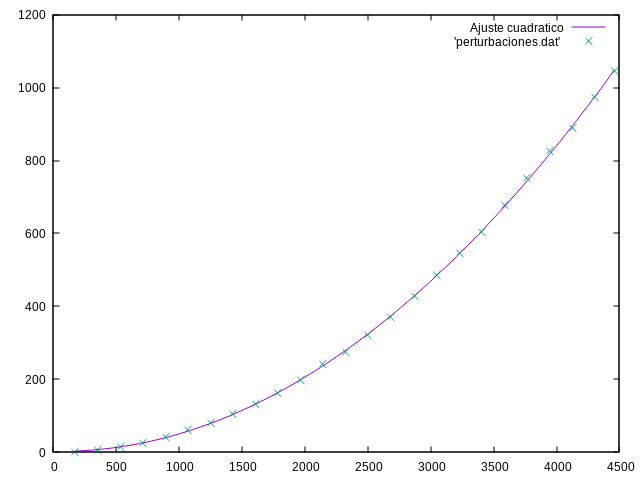
\includegraphics[scale=0.5]{./Images/perturbaciones.png}
 	\caption{Gráfica con los tiempos de ejecución del vecino más cercano. \(R^2 = 0.93507\)}
 \end{figure}
\end{frame}

\begin{frame}[fragile]{Heurística de perturbaciones. \normalfont{Resultados}}
\begin{itemize}
	\item \texttt{ulysses16.tsp}:
	\[
		[0,7,15,12,11,13,6,5,14,4,8,9,2,1,3,10] \qquad D = 101
	\]
	\item \texttt{bayg29.tsp}:
	\[
		[0,27,5,11,8,4,20,1,19,9,3,14,17,13,21,16,10,18,24,6,22,26,7,
	\]
	\[
		23,15,12,28,25,2] \qquad D = 10209
	\]
	\item \texttt{eil76.tsp}: Aplicando 10 perturbaciones, obtenemos que el mejor orden (teniendo en cuenta el orden del fichero original):
	\footnotesize
	\[
		[0,72,32,62,15,2,43,31,8,38,71,57,9,37,64,10,65,52,13,18,34,6,7,45,33,51,26,44,28,
	\]
	\[
		47,46,20,73,27,61,1,29,3,74,75,66,25,11,39,16,50,5,67,4,36,19,69,59,70,35,68,60,2,
	\]
	\[
		1,41,40,42,22,55,48,23,17,49,24,54,30,58,53,12,56,14,63] \qquad D = 642
	\]
	\normalsize
\end{itemize}
\end{frame}

\begin{frame}[fragile]{Heurística de perturbaciones. \normalfont{Gráficos}}
\begin{center}
\begin{tabular}{cc}
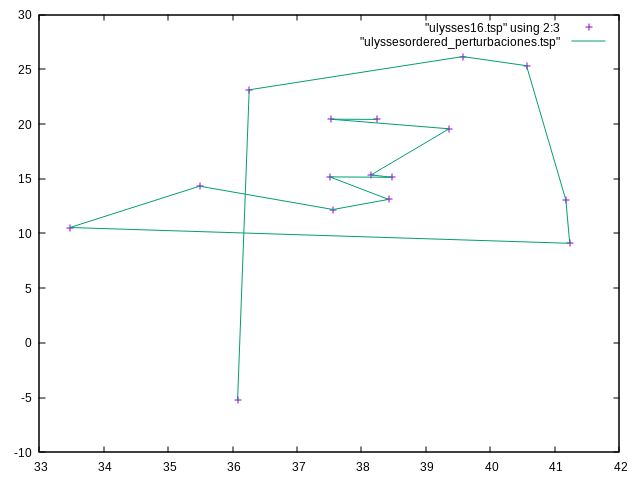
\includegraphics[scale=0.23]{./Images/ulysses_perturbaciones.png}
&
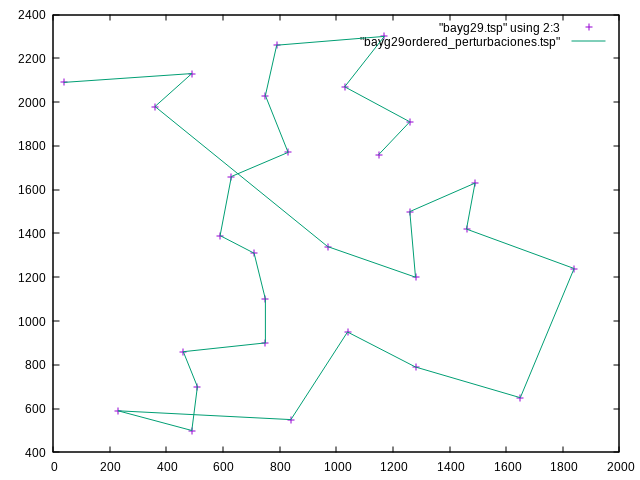
\includegraphics[scale=0.23]{./Images/bayg_perturbaciones.png} \\
Ulysses & Bayg
\end{tabular}
\end{center}
\begin{center}
\begin{tabular}{c}
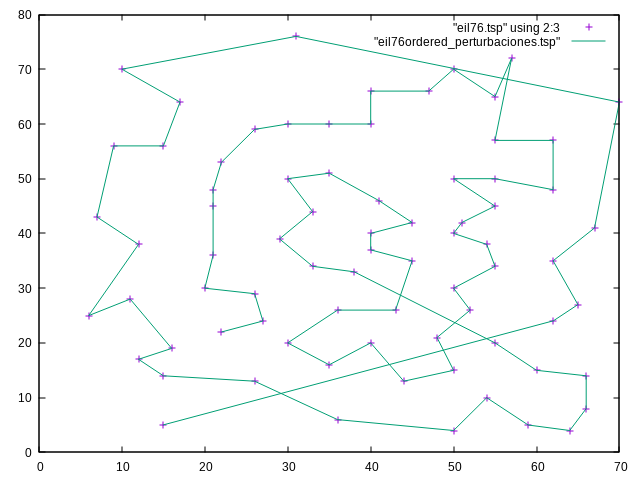
\includegraphics[scale=0.23]{./Images/eil_perturbaciones.png} \\
Eil
\end{tabular}
\end{center}
\end{frame}

\begin{frame}[fragile]{Comparación de las distinas heurísticas}
Los tres algoritmos que tenemos son: cercanía (el vecino más cercano), inserción y por perturbaciones. Veremos la gráfica comparativa de los tiempos de cada heurística.

\end{frame}
\begin{frame}[fragile]{Comparación de las distinas heurísticas}

\begin{figure}[h!]
 	\centering
 	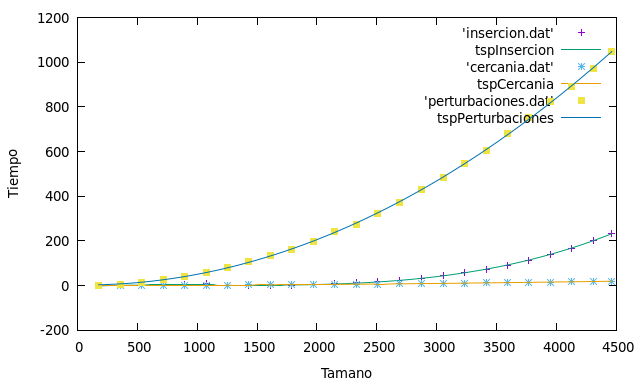
\includegraphics[scale=0.45]{./Images/comparativa_tiempos.png}
 	\caption{Gráfica comparativa con los tiempos de ejecución de las distintas heurísticas}
 \end{figure}

\end{frame}
 
 \begin{frame}[fragile]{Comparación de las distinas heurísticas}
\begin{table}[h!]
 	\centering
 	\footnotesize
 	\scalebox{0.5}{
 		\begin{tabular}{|c|c|}
 			\hline
 			\multicolumn{2}{|c|}{\textsf{Heurística de cercania}}
 			\\\hline
 			\bfseries Ciudades (n) & \bfseries Distancia ()
 			\csvreader{./data/cercania_distancias.csv}{}
 			{\\\hline\csvcoli&\csvcolii}
 			\\\hline
 		\end{tabular}
 	}
 	\scalebox{0.50}{
 		\begin{tabular}{|c|c|}
 			\hline
 			\multicolumn{2}{|c|}{\textsf{Heurística de insercion}}
 			\\\hline
 			\bfseries Ciudades (n) & \bfseries Distancia ()
 			\csvreader{./data/insercion_distancias.csv}{}
 			{\\\hline\csvcoli&\csvcolii}
 			\\\hline
 		\end{tabular}
 	}
 	\scalebox{0.50}{
 		\begin{tabular}{|c|c|}
 			\hline
 			\multicolumn{2}{|c|}{\textsf{Heurística de perturbaciones}}
 			\\\hline
 			\bfseries Ciudades (n) & \bfseries Distancia ()
 			\csvreader{./data/perturbaciones_distancias.csv}{}
 			{\\\hline\csvcoli&\csvcolii}
 			\\\hline
 		\end{tabular}
 	}
 	\caption{Experiencia empírica de las distintas heurísticas}
 \end{table}
 
 \end{frame}
 \begin{frame}[fragile]{Comparación de las distinas heurísticas}
 Vemos como los tiempos de ejecución son mayores para inserción debido a que su eficiencia es cúbica respecto a los demás, donde también se observa que la heurística de perturbaciones tiene un tiempo algo mayor que la de cercanía. Sin embargo este mayor tiempo se puede justificar a la hora de escoger estas heurísticas debido a que el algoritmo que proporciona mejores soluciones es, como se puede comprobar con los costes previamente reflejados, el que utiliza la heurística de inserción y posteriormente al que utiliza la heurística de perturbaciones. Por tanto la conclusión en este caso es que a mayor tiempo de ejecución mejor solución obtenemos y por tanto debemos de tener esto en cuenta a la hora de elegir una heurística u otra.
\end{frame}

\section{Conclusiones}

\begin{frame}[fragile]{Conclusiones}
	\begin{itemize}
		\item Los algoritmos Greedy nos ahorran la elevada complejidad de los algoritmos de fuerza bruta.
		\item Los algoritmos más eficientes no siempre son los más útiles.
		\item La anterior conclusión nos lleva a que debemos saber encontrar un término medio entre eficiencia y búsqueda de la solución óptima.
		\item Nos interesa una buena eficiencia y una solución próxima a la óptima
		\item Los algoritmos Greedy no siempre nos dan la mejor solución.
		
	\end{itemize}
\end{frame}

\end{document}